\chapter{Исследование линейного двухвходового дешифратора с инверсными входами}

Ниже, на рисунке \ref{fig:dc2-4}, представлена схема линейного двухвходового дешифратора с инверсными выходами.

\begin{figure}[ht]
	\centering
	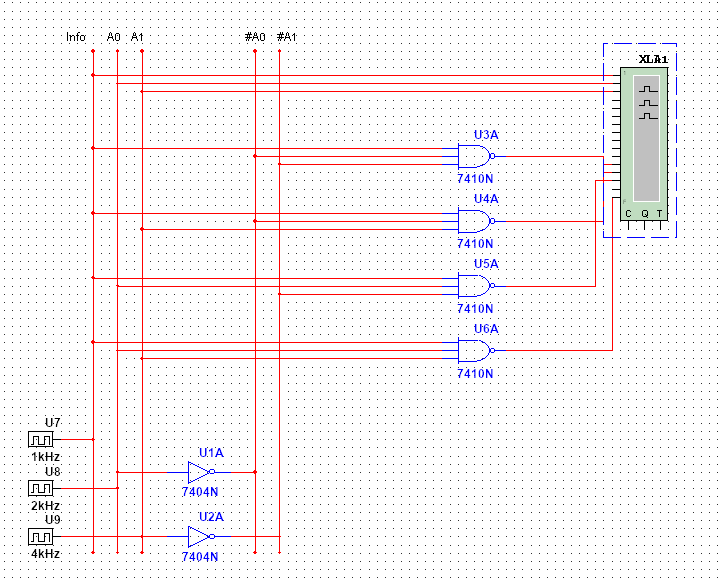
\includegraphics[width=\linewidth]{img/DC2-4}
	\caption{Линейный двухвходовый дешифратор}
	\label{fig:dc2-4}
\end{figure}

\pagebreak

Ниже, на рисунке \ref{fig:dc2-4-out}, представлена временная диаграмма сигналов исследуемого дешифратора.

\begin{figure}[ht]
	\centering
	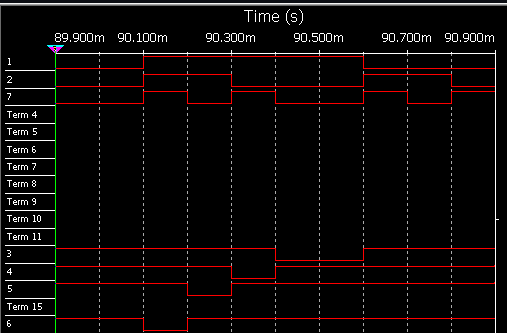
\includegraphics[width=0.6\linewidth]{img/DC2-4-out}
	\caption{Временная диаграмма сигналов дешифратора}
	\label{fig:dc2-4-out}
\end{figure}

Исходя из того факта, что дешифратор в программе Multisim является идеальным, устранение гонок сигнала не имеет смысла. В реальном дешифраторе необходимо, чтобы стробирующий сигнал не был равен единице во время переключения сигналов, причем надо учитывать время задержки $t_{lat}$. В случае линейного двухвходового дешифратора (рисунок \ref{fig:dc2-4}), время может быть высчитано по формуле \ref{eq:tlat}.

\begin{equation}
	\overline{t_{lat}} = \overline{t_{not}} + \overline{t_{nand}}
	\label{eq:tlat}
\end{equation}

Ниже представлена таблица переходов:

\begin{table}[ht]
	\centering
	\caption{Таблица переходов линейного двухвходового дешифратора с инверсными входами}
	\begin{tabular}{|c|c|c|c|c|c|c|}
		\hline
		$~~E~~$ & $~~A_1~~$ & $~~A_2~~$ & $~~F_1~~$ & $~~F_2~~$ & $~~F_3~~$ & $~~F_4~~$ \\
		\hline
		0 & $\forall$ & $\forall$ & 1 & 1 & 1 & 1 \\
		\hline
		1 & 0 & 0 & 0 & 1 & 1 & 1 \\
		\hline
		1 & 0 & 1 & 1 & 0 & 1 & 1 \\
		\hline
		1 & 1 & 0 & 1 & 1 & 0 & 1 \\
		\hline
		1 & 1 & 1 & 1 & 1 & 1 & 0 \\
		\hline
	\end{tabular}
\end{table}

\pagebreak

\chapter{Исследование дешифраторов ИС К155ИД4}

Ниже, на рисунке \ref{fig:2-74ls}, представлена схема двухвходового дешифратора ИС К155ИД4 (74LS155).

\begin{figure}[ht]
	\centering
	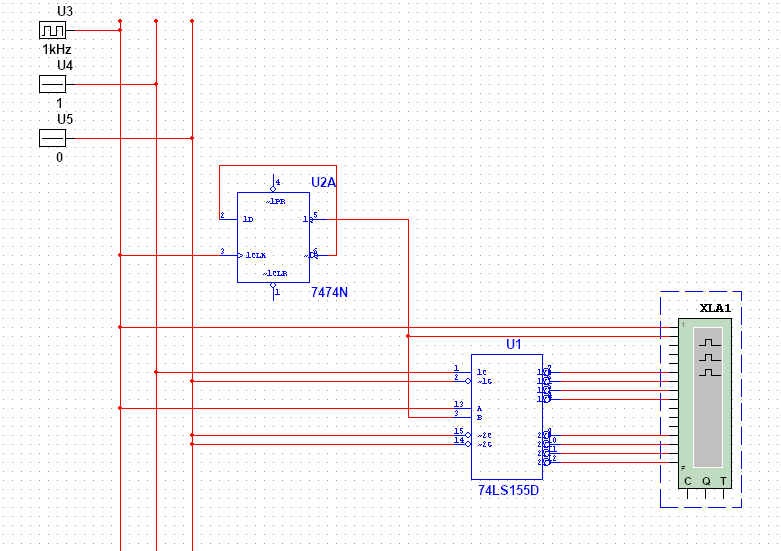
\includegraphics[width=\linewidth]{img/2-74LS}
	\caption{Схема двухвходового дешифратора ИС К155ИД4}
	\label{fig:2-74ls}
\end{figure}

\pagebreak

Ниже, на рисунке \ref{fig:2-74ls-out}, представлена временная диаграмма двухвходового дешифратора ИС К155ИД4 (74LS155).

\begin{figure}[ht]
	\centering
	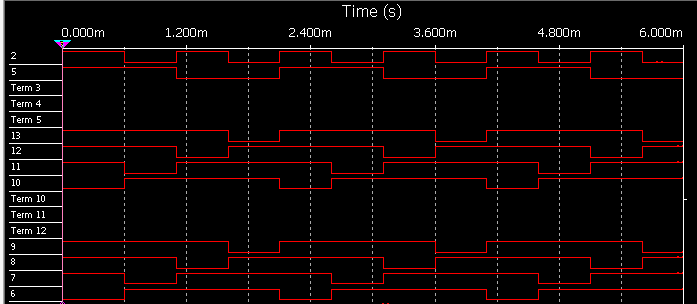
\includegraphics[width=0.7\linewidth]{img/2-74LS-out}
	\caption{Временная диаграмма сигналов дешифратора ИС К155ИД4}
	\label{fig:2-74ls-out}
\end{figure}

\pagebreak

Ниже, на рисунках \ref{fig:3-74ls1} и \ref{fig:3-74ls1-out}, приведены схема трехвходового дешифратора ИС К155ИД4 и временная диаграмма соответственно.

\begin{figure}[ht]
	\centering
	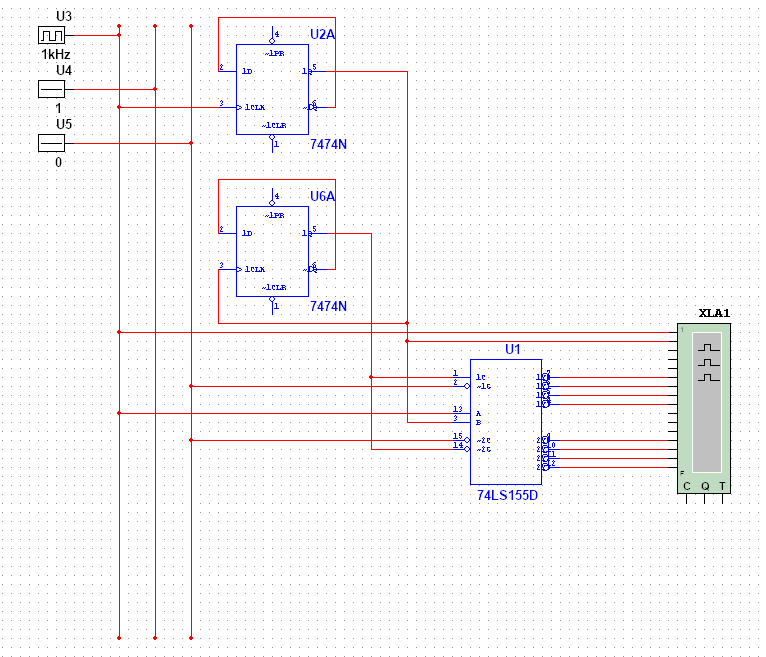
\includegraphics[width=\linewidth]{img/3-74LS1}
	\caption{Схема трехвходового дешифратора ИС К155ИД4}
	\label{fig:3-74ls1}
\end{figure}

\pagebreak

\begin{figure}[ht]
	\centering
	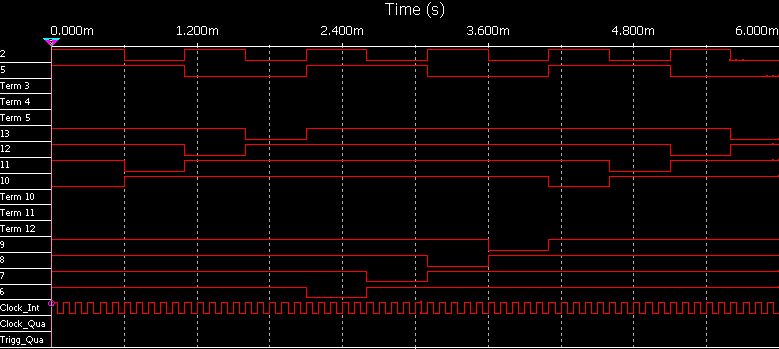
\includegraphics[width=0.7\linewidth]{img/3-74LS1-out}
	\caption{Временная диаграмма сигналов трехвходового дешифратора ИС К155ИД4}
	\label{fig:3-74ls1-out}
\end{figure}

Ниже представлена таблица переходов дешифратора ИС К155ИД4:

\begin{table}[ht]
	\centering
	\begin{tabular}{|c|c|c|c|c|c|c|c|c|c|c|c|}
		\hline
		$~~A_1~~$ & $~~A_2~~$ & $~~A_3~~$ & $~~F_1~~$ & $~~F_2~~$ & $~~F_3~~$ & $~~F_4~~$ & $~~F_5~~$ & $~~F_6~~$ & $~~F_7~~$ & $~~F_8~~$ \\
		\hline
		0 & 0 & 0 & 0 & 1 & 1 & 1 & 1 & 1 & 1 & 1 \\
		\hline
		0 & 0 & 1 & 1 & 0 & 1 & 1 & 1 & 1 & 1 & 1 \\
		\hline
		0 & 1 & 0 & 1 & 1 & 0 & 1 & 1 & 1 & 1 & 1 \\
		\hline
		0 & 1 & 1 & 1 & 1 & 1 & 0 & 1 & 1 & 1 & 1 \\
		\hline
		1 & 0 & 0 & 1 & 1 & 1 & 1 & 0 & 1 & 1 & 1 \\
		\hline
		1 & 0 & 1 & 1 & 1 & 1 & 1 & 1 & 0 & 1 & 1 \\
		\hline
		1 & 1 & 0 & 1 & 1 & 1 & 1 & 1 & 1 & 0 & 1 \\
		\hline
		1 & 1 & 1 & 1 & 1 & 1 & 1 & 1 & 1 & 1 & 0 \\
		\hline
	\end{tabular}
\end{table}


\chapter{Исследование дешифраторов ИС КР531ИД14}

\begin{figure}[ht]
	\centering
	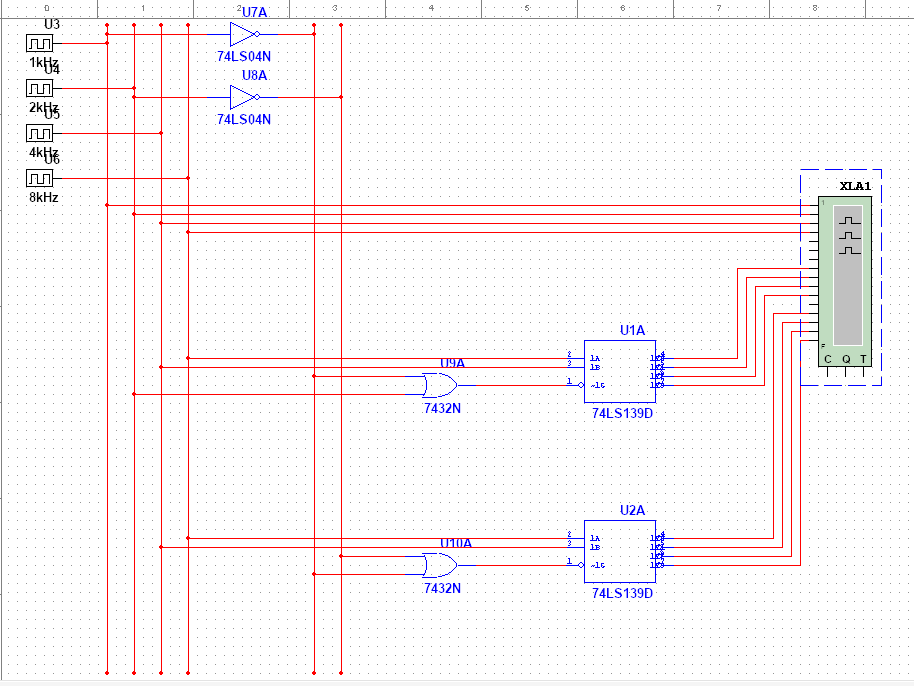
\includegraphics[width=1\linewidth]{img/DC3-8}
	\caption{Схема наращивания дешифраторов ИС КР531ИД14}
	\label{fig:dc3-8}
\end{figure}


\begin{figure}[ht]
	\centering
	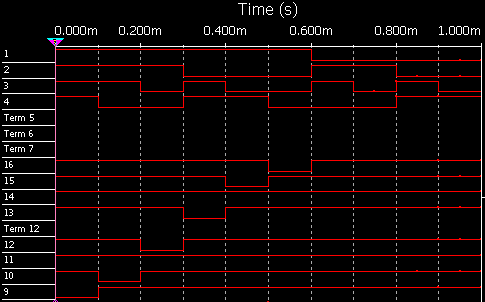
\includegraphics[width=0.7\linewidth]{img/DC3-8-out}
	\caption{Временная диаграмма композиции дешифраторов ИС КР531ИД14}
	\label{fig:dc3-8-out}
\end{figure}

\chapter{Исследование работоспособности дешифраторов ИС 533ИД7}

\begin{figure}[ht]
	\centering
	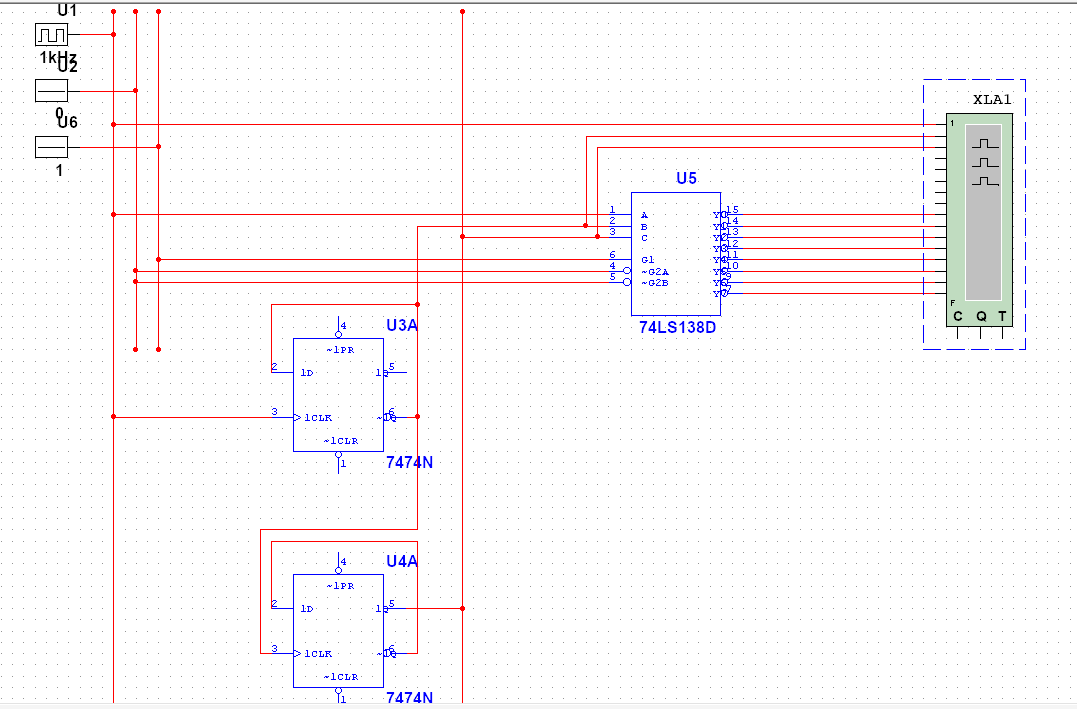
\includegraphics[width=1\linewidth]{img/DC3-8-solid}
	\caption{Схема трехвходного дешифратора ИС 533ИД7}
	\label{fig:dc3-8-solid}
\end{figure}


\begin{figure}[ht]
	\centering
	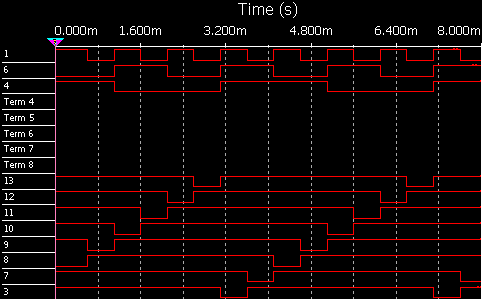
\includegraphics[width=0.7\linewidth]{img/DC3-8-solid-out}
	\caption{Временная диаграмма трехвходного дешифратора ИС 533ИД7}
	\label{fig:dc3-8-solid-out}
\end{figure}

